% Section facultative mais importante à mon avis

% 2 points clé : la méthodologie et pourquoi ce choix de technique
\section{Bayesian model}
\label{section:bayesmodel}
To solve this problem, the approach taken is a non-parametric Bayesian model based on the \textit{Hidden Markov Model} and a prior generated by a \textit{Hierarchical Dirichlet Process} (HDP-HMM). Since the basic HDP-HMM tends to over-segment the audio data which creates redundant states and rapidly switched among them, we describe an augmented HDP-HMM that provides effective control over the switching rate: the sticky HDP-HMM, a bayesian nonparametric hidden Markov models with persistent states. So we decided to 'augment' the method of the paper \cite{ren_dynamic_2010} by applying the method of \cite{fox_sticky_2011}. For this purpose, we want to segment a waveform into a set of time intervals with no \textit{a priori} on the number of intervals. The sequence is modelled using the Hidden Markov Model with the states to categorise the interval. In other words, we want the piece to be divided into intervals and each interval will be labelled to a state that we will later on analyse. For example a music piece can be divided into parts that are : intro, chorus, pre-chorus, outro. Those parts can be easily identified by the human ear and brain (music-theoretic analysis). We will compare our analysis to the results of the model. 

\begin{figure}[ht]
	\label{fig:waveform}
	\centering
  	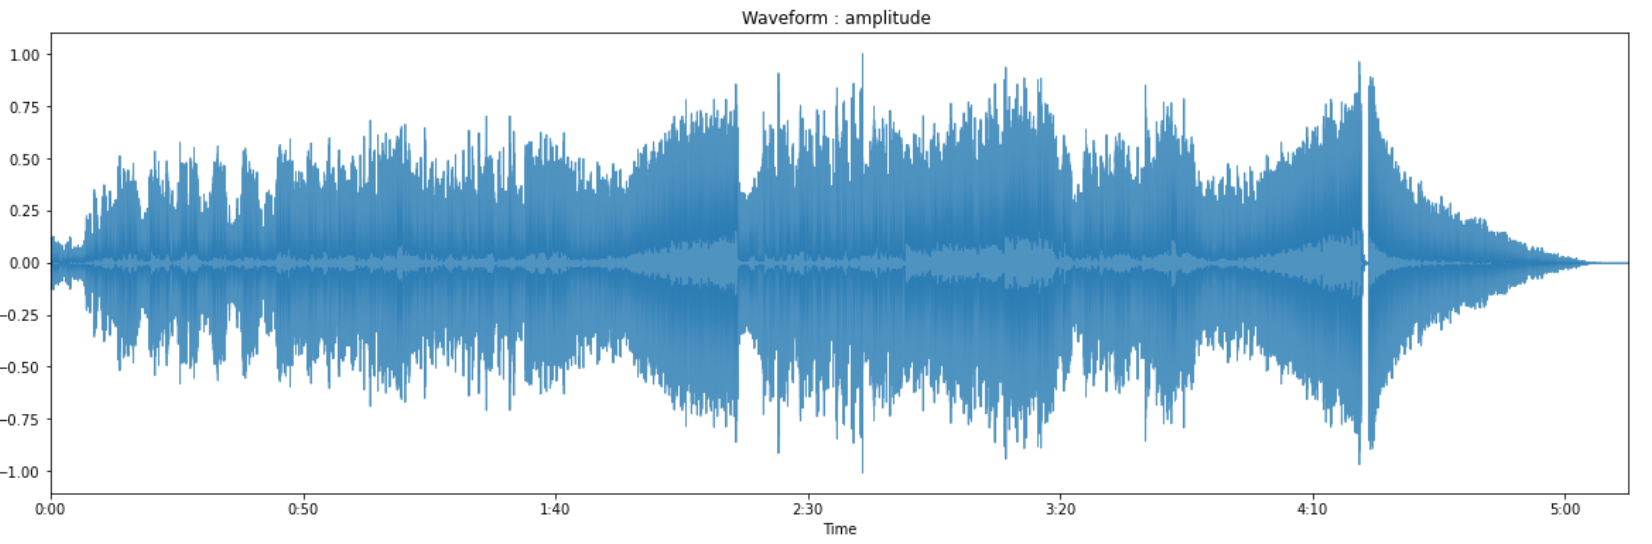
\includegraphics[scale=0.25]{Graphics/Audio/waveform2} 
   	\caption{Audio waveform of the piece considered}
\end{figure}

\subsection{Hidden Markov Model}
The Hidden Markov Model used is described as follows : A discrete sequence of observed data $y=\{y_t\}^T_{t=1}$ with $y_t \in \{1,\dots, M \}$ and a corresponding hidden state sequence $s=\{s_t\}^T_{t=1}$ with $s_t \in \{ 1, \dots, I \}$. The states will be analysed as in Section \ref{section:bayesmodel} (intro, chorus, etc.). Each observation is associated to a state. The discrete HMM model is represented by its parameters $\theta=\{\pi,B,A\}$ such that : 
\begin{itemize}
	\item $\pi$ is a set of state transition probabilities, the probability to transition from one state to another.For two states $\rho$ and $\xi$, the transition probability from $\rho$ to $\xi$ is $\pi_{\rho\xi}=\mathbb P(s_{t+1}=\xi | s_t=\rho)$
	\item $B$ is a set of emission probabilities, the probability that an observation associated to a state $\rho$ is equal to $m$ : $b_{\rho m}=\mathbb P(x_t= m | s_t=\rho)$
	\item  $A$ is the set of initial state distribution, the probability that the first observation in time $t=1$ is equal to the state $\rho$ : $a_{\rho}=\mathbb P(s_1=\rho)$
\end{itemize}
Because we will use a Hierarchical Dirichlet Process to model the parameters $\theta$, we will divide the sequence into $J$ subsequences. This means that we will model J Hidden Markov Models. By taking the notation at the beginning of this section, we will have $j\in \{1, \dots, J\}$ and $y=\{y_j\}_{j=1}^J$ with $y_j=\{ y_{ji}\}_{i=1}^{N_j}$. Note that every subsequence $x_j$ has a length $N_j$. We allow the parameters to be different in each subsequence such that : \begin{align*}
 		x_j \sim HMM(\theta_j)
 \end{align*}
The joint distribution given $\theta$ is : 
\begin{align*}
	p(y|\theta)=\prod^J_{j=1}\left\{ \sum_{s_j}a_{s_{j,1}}\prod^{N_j-1}_{i=1}\pi_{s_{j,i+1}} \prod^{N_j}_{i=1} b_{s_{j,i}y_{j,i}} \right\}
\end{align*} \\

\subsection{Sticky Hierarchical Dirichlet Process}
A Hierarchical Dirichlet Process is defined as a collection of Dirichlet Processes. Our collection of DP processes is the J parameters $\theta_j$ linked to the HMM. This kind of setting allows for analysing how inter-related are the subsequences one to the others. The first process of the collection is denoted as : 
\begin{align*}
	G_0\sim DP(\gamma, H)
\end{align*}
with $\gamma$ a concentration parameter for the Dirichlet distribution which is symmetrical and H a base probability measure on $\Theta$. The formal definition of a Dirichlet process is $\forall (B_k)_{k=1,\dots, K}$ finite partition of $\Theta$ : \begin{align*}
	(G_0(B_k))_{k=1,\dots, K}|\gamma, H \sim Dir( (\gamma H(B_k))_{k=1,\dots, K})
\end{align*}
We approach the Dirichlet Process with a stick-breaking process and we can write $G_0$ as follows :
\begin{align*}
	G_0=\sum^\infty_{k=1} \beta_k \delta_{\theta_k}
\end{align*}
with $\delta_{\theta_k}$ an indicator function in $\theta_k$ and $\beta_k$ the mixture weights computed such that :
\begin{align*}
\beta_k &\sim Stick(\gamma) \\
	\beta_k&= v_k\prod^{k-1}_{l=1}(1- v_l) \\
	v_k&\sim Beta(1, \gamma)
\end{align*}
with $v_k$ the independent random variables following a Beta distribution. The process to obtain the probabilities $\beta_k$ is pictured as breaking a unit-length stick because we start off with a stick of length 1 and at each step we  we break a portion of the what is remaining stick according to $v_k$ and assign to $\beta_k$ the piece broken. The smaller the $\alpha$ the more concentrated is the distribution. The first process $G_0$ (first subsequence) is then used as the base measure for the other processes (other subsequences) : 
\begin{align*}
	G_j &\sim DP(\alpha, G_O) \\
	G_j &= \sum^\infty_{t=1}\tilde{\pi}_{jt} \delta_{\theta^\star_{jt}} \\
	\tilde{\pi}_{j}| \alpha &\sim Stick(\alpha) \\
	\theta^\star_{jt}|G_0 &\sim G_0 \\
	\theta_{ji}'|G_j &\sim G_j \\
	y_{ji} |\theta'_{ji} &\sim F(\theta'_{ji})\end{align*} 
with $j\in \{1,\dots, J\},\ i\in \{ 1,\dots, N_j\}$. We know that multiple $\theta^\star_{jt}$ can take the same value $\theta_k$. We can write $G_j$ as a function of unique states :
\begin{align*}
	G_j &\sim \sum^\infty_{k=1} \pi_{jk} \delta_{\theta_k} \\
	\pi_j|\alpha, \beta  &\sim DP(\alpha, \beta) \\
	\theta_k |H &\sim H
\end{align*}
with $\pi_{jk}$ the distribution of the subsequence $j$ over the state $k$ with : 
\begin{align*}
	\pi_{jk} = \sum_{t|\theta^\star_{jt}= \theta_k} \tilde{\pi}_{jt}
\end{align*}
The model can be re written with an indicator variable $z_{ji}$ for the state assigned to the observation $y_{ji}$ : 
\begin{align*}
	G_j &\sim DP(\alpha, G_O) \\
	z_{ji}|\pi_j &\sim \pi_j \\
	y_{ji}| \{\theta_k\}, z_{ij} &\sim F(\theta_{z_{ji}})
\end{align*}
With $F(\cdot)$ the fixed distribution of the data sample. According to \cite{fox_sticky_2011}, we compute a sticky version of the model by adding a $\kappa$ parameter that will slow down the transitions between states and avoid having unrealistically fast dynamics as results. The new transition distributions are modelled as follows : 
\begin{align*}
	\beta|\gamma &\sim Stick(\gamma) \\
	\pi_j| \alpha, \kappa, \beta  &\sim DP\left(\alpha + \kappa, \frac{\alpha\beta + \kappa \delta_j}{\alpha + \kappa} \right) 
\end{align*}
By adding this parameter, we are increasing the probability of self-transition by an amount proportional to k. If the probability that an observation has the same state as the one after is higher, the changing dynamics will slow down. That is why the $\kappa$ parameter is added on the $j^{th}$ component of $\alpha\beta$. \\

\section{Computational method}
% 2 points clé : la description de la méthode et les difficultés rencontrées
We use the \textit{Gibbs Block Sampler} \cite{fox_sticky_2011} for the inference of the parameters of the sticky HDP-HMM. The first step is to sample $\beta$ and $\pi$. The sampler is defined with a finite Dirichlet prior on $\theta_j$ such that : 
\begin{align*}
	\beta | \gamma \sim Dir(\gamma/L, \dots, \gamma/L) \\
	\pi_j | \alpha, \beta \sim Dir (\alpha\beta_1, \dots, \alpha\beta_L)
\end{align*}
This finite approximation is made because when $L\to\infty$ then it converges to the HDP mixture model. The derived posterior distribution is : 
\begin{align*}
	\beta|\bar{n},\gamma &\sim Dir(\gamma/L+\bar m_{\cdot1}, \dots, \gamma/L+ \bar m_{\cdot L}) \\
	\pi_j | z_{1:T},\alpha, \beta &\sim Dir(\alpha\beta+n_{j1}, \dots, \alpha\beta_j+\kappa + n_{jj}, \dots, \alpha \beta_L+n_{jL})
\end{align*}
with $n_{jk}$ the number of j to k transitions in the state sequence j.
The choice of initialisation of the base measure is made regarding the paper \cite{fox_sticky_2011} with :  
\begin{equation}
	\label{equ:basemeasure}
\begin{split}
	y|z=k&\sim \mathcal N (\mu_k, \sigma_k^2) \\
	\mu_k &\sim \mathcal N (0, s^2) \\
	\sigma^2_k &\sim InvGamma(a,b)
\end{split}
\end{equation}

After, choosing the hyper-parameters and base measure, the next step is to sample the hidden states $z_t$. This is done with a forward-backward algorithm to jointly sample $z$ given $y$ for the sticky HDP-HMM. The conditional distribution is : 
\begin{align*}
	p(z|y, \pi, \theta) = p(z_t|z_{t-1}, y, \pi, \theta) p(z_{t-1}|z_{t-2}, y, \pi, \theta) \dots p(z_2|z_1 y, \pi, \theta) p(z_1| y, \pi, \theta) 
\end{align*} 
The algorithm starts by sampling $z_1$ from $ p(z_1| y, \pi, \theta)$ then sample $z_2$ from $ p(z_2|z_1, y, \pi, \theta)$ and so on. The conditional distribution is :\begin{align*}
	 p(z_1| y, \pi, \theta) &\propto p(z_1)f(y_1|\theta_{z_1})\sum_{z_{2:T}} \prod_t p(z_t|\pi_{z_{t-1}})f(y_t|\theta_{z_t})\\&\propto  p(z_1)f(y_1|\theta_{z_1}) \sum_{z_2}p(z_2|\pi_{z_1})f(y_2|\theta_{z_2})m_{3,2}(z_2)
	 \\ &\propto  p(z_1)f(y_1|\theta_{z_1})m_{2,1}(z_1)
\end{align*}
where $m_{t,t-1}(z_{t-1})$ is called the \textit{bakward message} passed from $z_t$ to $z_{t-1}$ and defined by : 
\begin{align*}
	m_{t,t-1}(z_{t-1}) \propto p(y_{t:T}|z_{t-1},\pi,\theta)
\end{align*}
In the algoritm the messages are first initialized to :\begin{align*}
	m_{T+1,T}(k)=1
\end{align*}
and then with a backward loop for each $k\in \{1,\dots, L\}$ we compute the messages : \begin{align*}
	m_{t,t-1}(k)&=\sum^L_{j=1}\pi_k(j) \mathcal N(y_t, \mu_j, \Sigma_j)m_{t+1, t}(j)\\
	&=\sum^L_{j=1}\pi_k(j) \frac{1}{\Sigma_j}\exp\left[ -\frac{1}{2} \left( \frac{y_t-\mu_j}{\Sigma_j}\right)^2\right]m_{t+1, t}(j)
\end{align*}
Because of (\ref{equ:basemeasure}) we have $\mathcal N(y_t, \mu_j, \Sigma_j)\propto \frac{1}{\Sigma_j} e^{-\frac{1}{2} \left( \frac{y_t-\mu_j}{\Sigma_j}\right)^2}$.Then we derive the general distribution for $z_t$ which is : 
\begin{align*}
	p(z_t|z_{t-1}, y, \pi,\theta) \propto p(z_t|\pi_{z_{t-1}})f(y_t|\theta_{z_t})m_{t+1,t}(z_t)
\end{align*}
The algorithm computes the $z_t$ with a forward loop  with for each $(j,k)\in \{1,\dots, L\}^2$ computes the probability of $y_t|z_t=k$:
\begin{align*}
	f_k(y_t)=\pi_{z_{t-1}}(k)\mathcal N (y_t,\mu_k,\Sigma_k)m_{t+1,t}(j)
\end{align*}
and then assigns a state $z_t$ if the probability of having $y_t$ conditional to the state $k$ is inferior to the probability conditional to the state $j$  : $f_k(y_t)<f_j(y_t)$ then the state in $t$ is updated $z_t=j$ and we eventually update the transition matrix (N). \\

The next step is to sample the auxiliary variables. They are introduced to simplify the inference algorithm. Those random variables are the following : \begin{align*}
	w_{jt}|\alpha, \kappa \sim Ber\left( \frac{\kappa}{\alpha+\kappa} \right) \\ 
	\bar k_{jt} | \beta \sim \beta 
	\\ 
	k_{jt} | \bar k_{jt} , w_{jt} = \begin{cases}
		\bar k_{jt}, & w_{jt} =0 \\ j, & w_{jt} =1
	\end{cases}
\end{align*}
With $k_{jt}$ the state actually assigned, $\bar k_{jt}$ a considered state and $w_{jt}$ an override variable that can override the considered state and be assigned instead. This will allow for the $\kappa$ parameter to be taken into account for the "stickiness" of the model. We want 

We have to consider the number of observations that are transitioning from state $j$ to $k$ and for each transition $n_{jk}$ the probability that an observation actually transitions is given by a Bernoulli random variable :\begin{align*}
	Ber\left(\frac{\alpha\beta_k+\kappa\delta(j,k)}{n+ \alpha \beta_k+ \kappa \delta(j,k)} \right)
\end{align*}
For $i = 1,\dots,n_{ij}$ we sample the random variable and increment the count $m$ when the variable is equal to 1, then $m_{jk}$ follows a Binomial distribution :
\begin{align*}
		m_{jk} \sim Binomial\left(n_{jk},\:\frac{\alpha\beta_k+\kappa\delta(j,k)}{n+ \alpha \beta_k+ \kappa \delta(j,k)} \right)
\end{align*}
Then for each $j\in \{1,\dots,L\}$ we sample the number of override variables $w_{j\cdot}$ in state j. 
\begin{align*}
	w_{j\cdot}\sim Binomial\left( m_{jj}, \frac{}{} \right) 
\end{align*}

\section{Data processing}
We consider an acoustic signal in a mp3 format loaded in Python using the librosa package. The sampling rate is 22.05kHz which means we have 22050 observations par second of audio signal. The acoustic signal is first loaded as a waveform or amplitude as shown in Figure \ref{fig:waveform}. It represents the pressure change recorded by a recording instrument such as a microphone. We then divide the piece into 100ms contiguous frames. Each amplitude frame is processed by computing its Mel frequency sceptral coefficients (MFCCs). These coefficients are derived from the Melspectrogram that is a log-scale of pitches judged to be equally distanced to one another. The Mel spectrogram is the representation showing the mel frequencies according to time and intensity. The MFCCs are the most popular feature used in audio processing. We compute 40 columns of coefficients for each frame. To obtain a vector sequential data, we quantize each frame of coefficient. First, we \textit{whiten} the columns so each one of them have a unit variance. Indeed, before running k-means agorithm, we need to rescale each feature dimension of the observations by the standard deviation. Then we use the k-means algorithm with 16 centroids to generate to adjusts the classification of the observations into clusters and updates the clusters centroids until the position of the centroids is stable over successive iterations. This yields a code book mapping centroids to codes and vice-versa. After that, we pass them to the vector quantization algorithm which assigns codes from a code book to observations. The result is a 1D discrete sequential data representing the coefficients. After the piece is processed, the sequence is represented as a series of discrete observations. According to the paper, we should have the following figure which represents each observation by its cluster discretization. 
\begin{figure}[h]
    \label{fig:output}
    \centering
  	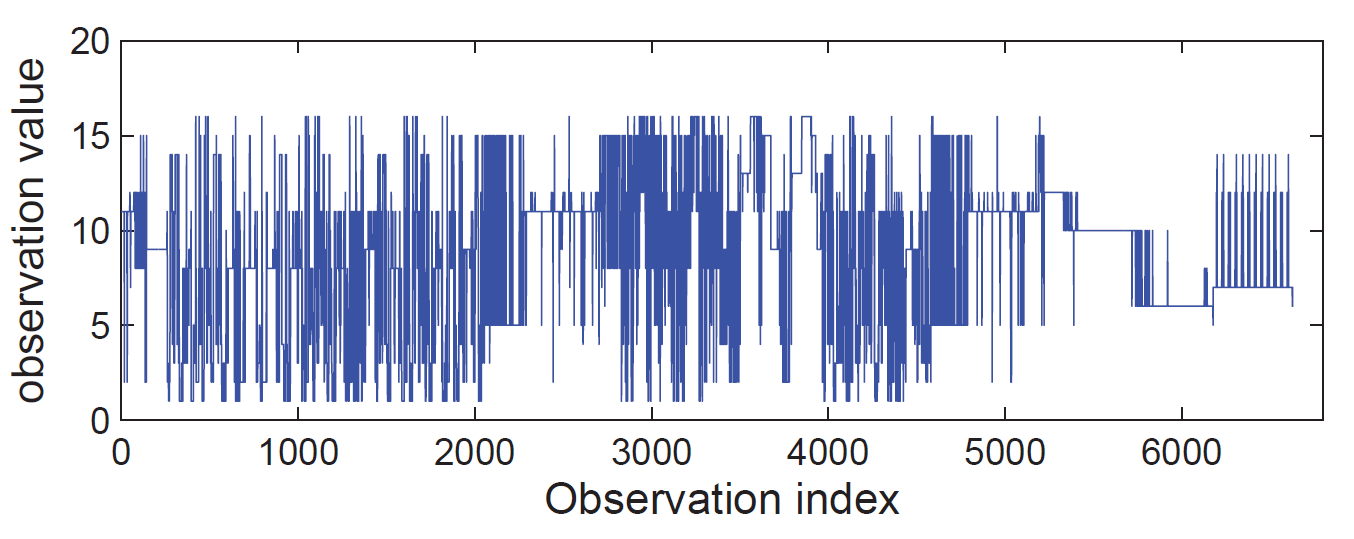
\includegraphics[scale=0.25]{Graphics/output.PNG} 
   	\caption{Sequence of code indices for the Beatle's music using a codebook of dimension $M = 16$}
\end{figure}

Unfortunately, after a lot of attempts, we've never managed to find this plot. After the discretization using k-means and Vector Quantization, we find the following plot:
\begin{figure}[h]
    \centering
  	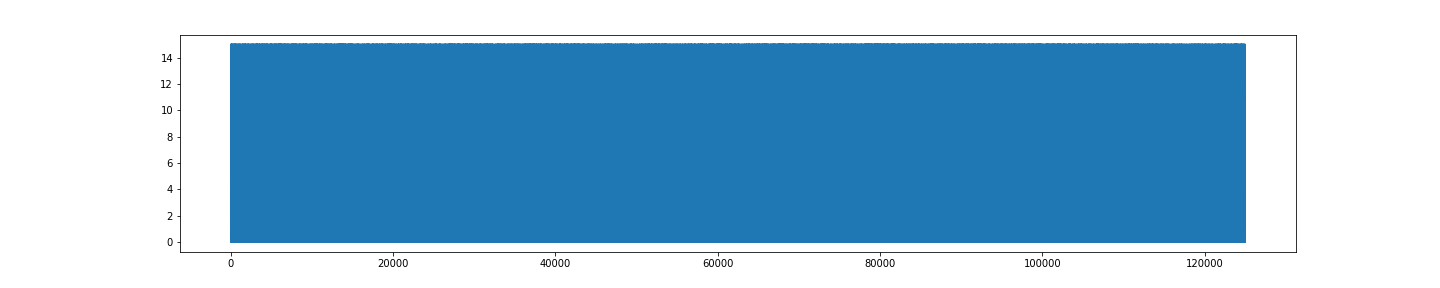
\includegraphics[scale=0.25]{Graphics/ouroutput.PNG} 
   	\caption{Our output}
\end{figure}

Indeed, the paper doesn't give enough details about the pre-processing part. We tried to use other papers from the same author, about the same topic, to see if he's giving some other details but we didn't succeed. So, we decided to use simulated data to apply our bayesian model. We found them online in the Github of a similar topic.

\section{Results}
Since our results are not interpretable, we propose to analyze the results of the research paper studied. As we said, after the piece is processed, the sequence is represented as a series of discrete observations as we showed in Figure \ref{fig:output}. Then, we divided the piece into 88 subsequences of 75 observations. The music segmentation results using dHDP HMM model is shown in the following figure : 
\begin{figure}[h]
    \centering
  	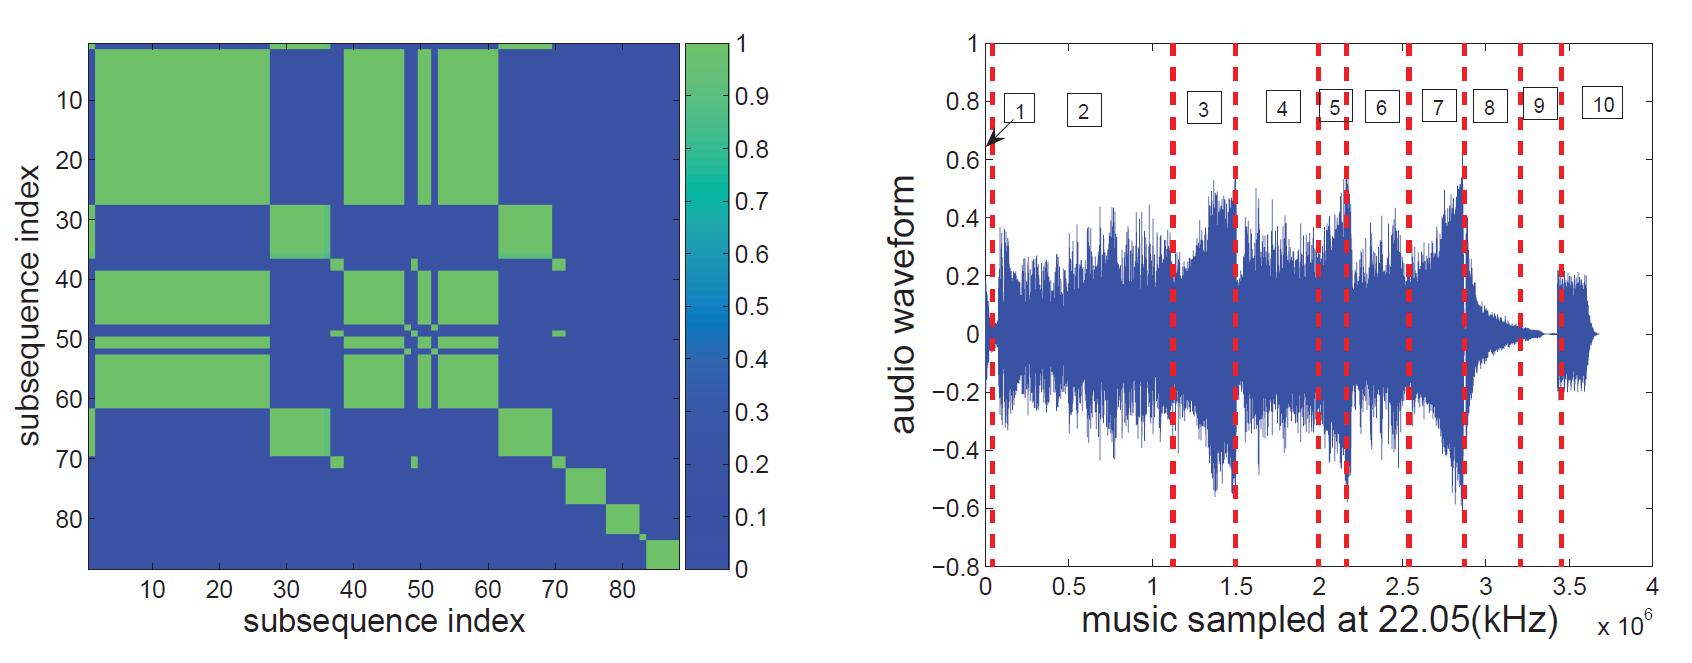
\includegraphics[scale=0.32]{Graphics/results.PNG} 
   	\caption{Paper results}
\end{figure}

The first plot is the similarity matrix $E(z^{'}z)$. It quantifies how inter-related any one subsequence of the music is to all others. The second one is the segmentation result on the Beatles audio waveform \ref{fig:waveform}. We can see that the audio is decomposed into clear segments of various lengths and some of them are repeated. To analyse the second plot, we have to compare these segments with a music-theoric analysis of the same audio. This method will allowed us to compare the results of our model and the segmentation done by a person.

\begin{figure}[h]
    \label{fig:segmentation}
    \centering
  	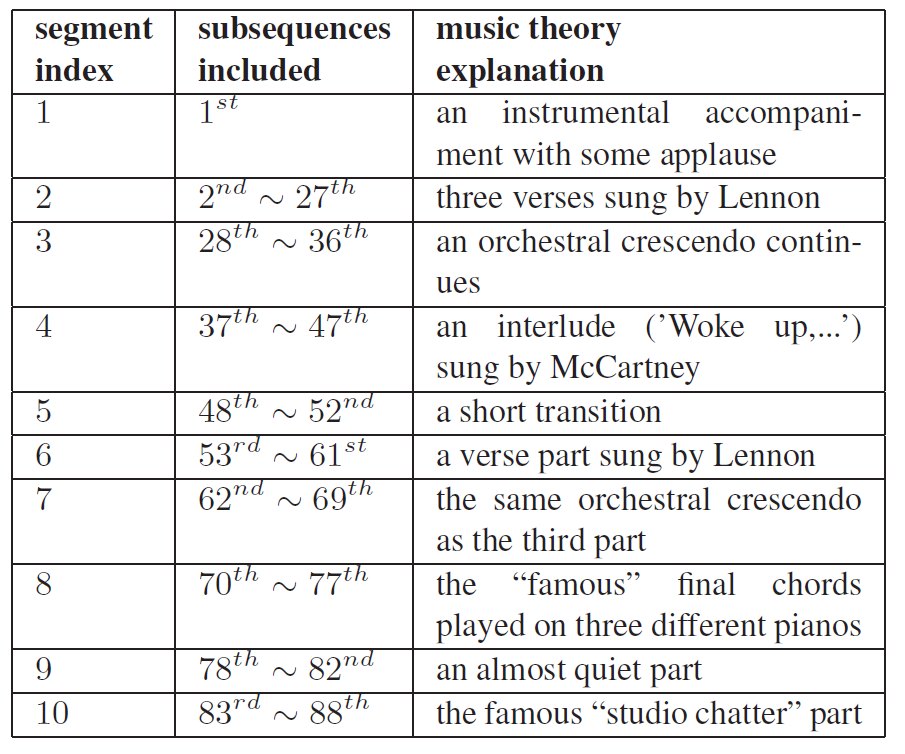
\includegraphics[scale=0.32]{Graphics/segmentation.PNG} 
   	\caption{Paper results}
\end{figure}

As we see, the segmentation is almost the same. Our music audio is divided into 10 parts with some redundant segments corresponding to the choruses. Each segment represents a specific part of the music: the verse of a singer, the instrumental part,... 